\cotefile{156-8}
\scanpage{121}
\mspage{112}
% archive sheet number: 121

Regardons l'opération \unsure{suiv.} $\unsure{A}$ sur $\Phi$
\diagram{
\footnotesize
\begin{tikzcd}[ampersand replacement=\&,column sep=small,row sep=small]
\Phi \arrow[r,mapsto] \&
\overline{\Phi} \arrow[r,mapsto] \&
\underbrace{\overline{\Phi}\setminus\underset{\substack{\Vert\\\Phi_{\mathrm{is}}}}{\overline{\Phi}_{\mathrm{is}}}}_{\substack{\text{adhérence}\\\text{purement}\\\text{1-dimensionnelle}}}
\arrow[r,mapsto,double,shorten <=2pt] \&
\Phi_{\deleted{\unsure{\mathrm{t\acute elescope}}}\mathrm{conv}}=\boxed{\Psi}
\\
\& \begin{gathered}\text{\uline{figure}}\\
\text{\uline{\unsure{enveloppante}}}\\
\deleted{\unsure{\mathrm{associ\acute ee}}}\deleted{\unsure{\Phi}}\ \text{de}\\
\Phi,\ \text{\uline{ou adhérence}}
\end{gathered}
\&
\& \begin{gathered}\text{ou ``\deleted{\unsure{télescopage}}}\\
\text{\inserted{\unsure{complétion|contraction}}}\\
\text{par effacement}\\\text{des pts ordinaires}\\
\text{de }\overline{\Phi}\setminus\overline{\Phi}_{\mathrm{is}}\text{''}
\end{gathered}
\end{tikzcd}}

On trouve une figure dont les composantes connexes sont des segments, donc donnée par une \deleted{suite} drapeau dans $\unsure{\mathcal{M}|M}_1$, ordonné par $\deleted{\unsure{\lhd}}\lhd$
\[
\begin{aligned}
D&\in\mathrm{Drap}^{*}(\mathcal{M}_1,\lhd)\\
\Big\Vert\quad&\\[-1.5ex]
\{X_1,X_2,\ldots X_n\}&
\end{aligned}
\]
\[
\text{\unsure{``}}\qquad X_i=\unsure{S|\mathscr{S}}_{a_i,b_i}\,,
\]
\figure{
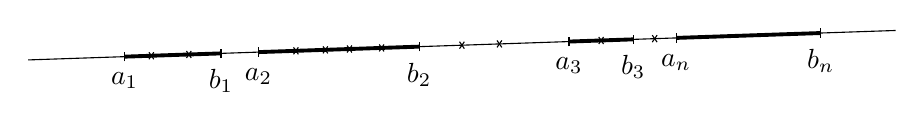
\begin{tikzpicture}[x=.68cm,y=.68cm]
\draw[thin] (0,0)--(16.2,.55);
\draw[line width=1.4pt] (1.8,.061)--(3.6,.122);
\draw[line width=1.4pt] (4.3,.146)--(7.3,.248);
\draw[line width=1.4pt] (10.1,.343)--(11.3,.384);
\draw[line width=1.4pt] (12.1,.411)--(14.8,.502);
\foreach \x/\y/\lab in {1.8/.061/a_1,3.6/.122/b_1,4.3/.146/a_2,7.3/.248/b_2,10.1/.343/a_3,11.3/.384/b_3,12.1/.411/a_n,14.8/.502/b_n}{
\draw (\x,\y-.09)--(\x,\y+.09);
\node[below] at (\x,\y-.12) {$\lab$};}
\foreach \x/\y in {2.3/.078,3/.102,5/.17,5.55/.188,6/.204,6.6/.224,8.1/.275,8.8/.299,10.7/.363,11.7/.397}{
\draw (\x-.045,\y-.065)--(\x+.045,\y+.065);
\draw (\x-.045,\y+.065)--(\x+.045,\y-.065);}
\end{tikzpicture}}

de telle façon que
\[
\left\{\begin{aligned}
\Psi=\Phi_{\mathrm{conv}}&=\Phi_D=\Phi_{X_1,X_2,\ldots,X_n}\\
\delta\deleted{\unsure{\Phi}}\Psi_{\deleted{\unsure{\mathrm{conv}}}}\inserted{{}=\delta\Psi}&=\partial\Phi=\{a_1,b_1,a_2,b_2,\ldots,a_n,b_n\}.
\end{aligned}\right.
\]

Pour \deleted{en donner} décrire $\Phi$ en termes de $\Phi_{\deleted{\unsure{\mathrm{comp}|\mathrm{conv}}}\mathrm{conv}}$ il faut :

1°) Donner $\inserted{\boxed{\Delta}}\unsure{\delta|\partial}\Phi=\ \in\mathrm{Drap}^{*}(\unsure{\mathcal{L}|L})\supset\unsure{\delta|\partial}\Psi$

\hspace*{1em}drapeau de $\mathcal{L}$ contenant $\delta\Psi$.

Les nouveaux pts rajoutés\textsuperscript{*} sont donc \unsure{juste} les \deleted{points} sommets isolés et les sommets internes de $\Phi$.
% slanted
\margin{\textsuperscript{*}\unsure{marqués} par un $\times$}
\scanpage{122}
\mspage{113}
% archive sheet number: 122

\deleted{2°) Dans $\delta\Psi=\partial\Psi$,}

Les sommets \deleted{isolés sont} internes sont \deleted{ceux de}\inserted{les} éléments de
\[
\Delta_{\mathrm{int}}=(\Delta\deleted{\unsure{\epsilon}}\setminus\partial\Psi]\cap\mathrm{Omb}(\Psi)=\Delta\cap\mathrm{Omb}^{\circ}(\Psi)
\]
Les sommets isolés sont \deleted{ceux de} les autres sommets $\deleted{\Delta\setminus\partial\Psi}$ de $\Delta\setminus\partial\Psi$,
\[
\Delta_{\mathrm{is}}=\deleted{\unsure{\Delta\setminus(\partial\Psi\cup\Delta}}(\Delta\setminus\partial\Psi)\setminus\Delta_{\mathrm{int}}
\]
\deleted{2°) \unsure{Distinguer}, \unsure{donc donner}, dans $\Delta_{\mathrm{int}}$,}
\deleted{une partie}
donc on a une décomposition
\[
\Delta=\partial\Psi\amalg\Delta_{\mathrm{int}}\amalg\Delta_{\mathrm{is}}
\]

2°) Se donner, dans $\Delta_{\mathrm{int}}$, les sommets qui appartiennent à $\Phi_0$ (sommets internes propres, ou sommets de \unsure{redondance} ou de \unsure{morcèlement|morcellement}), ou ce qui revient au $=$, les autres : \unsure{les} sommets lacunaires
\[
\boxed{\Delta_{\mathrm{lac}}}\subset\Delta_{\mathrm{int}}
\]
de sorte que
\[
\Delta_{\mathrm{int}}=\Delta_{\mathrm{lac}}\amalg\Delta_{\mathrm{red}}\,.
\]

3°) Dans $\partial\Psi$\inserted{$(=\partial\Phi)$}, dire quels sommets sont dans $\Phi_0$ \deleted{et lesquels} (sommets bords propres de $\Phi$) et lesquels non, i.e. se donner une partie
\[
\begin{aligned}
&\deleted{\unsure{\partial_0\Psi|\delta_0\Psi}}\\
&\unsure{\partial_0|\delta_0}\subset\partial\Psi\,.
\end{aligned}
\]

En résumé :
\scanpage{123}
\mspage{114}
% archive sheet number: 123

\uline{Proposition} Une préfigure quelconque est déterminée par les données suivantes

\unsure{4°|1°}) Une figure \textcircled{$\Psi$}\inserted{sans sommets isolés et} à composantes connexes des \deleted{multi} segments, \inserted{\deleted{(i.e. $\delta\Psi=\partial\Phi$} i.e. telle que $\delta\Psi=\partial\Phi$)} déterminée par
\[
D=(X_1\lhd X_2\lhd\deleted{\unsure{X_3}}\ldots X_n)\in\mathrm{Drap}^{*}(\unsure{\mathcal{M}|M}_1).
\]
\deleted{2°) Une}
\deleted{tel} que
\[
\Psi=\Phi_D=\bigcup_{X\in D}\widetilde{X}_{\deleted{\unsure{i}}}=\bigcup_{1\leq i\leq n}\widetilde{X}_i
\]
(réunion \unsure{disjoint|disjointe}). On aura
\[
\partial\Psi=\delta\Psi=\bigcup_{X\in D}\partial X=\bigcup_{1\leq i\leq n}\partial X_i
\]
(réunion disjointe), soit
\[
\delta\Psi=\{a_1,b_1,a_2,b_2,\ldots,a_n,b_n\}
\]
si
\[
\partial X_i=\{a_i,b_i\}\,.
\]

On peut dire aussi que $\Psi$ est déterminée par une suite \unsure{strict\textsuperscript{t}} croissante de cardinal pair
\[
a_1<b_1<a_2<b_2\ldots<a_n<b_n\,,
\]
et on aura
\[
X_i=\unsure{S|\mathscr{S}}_{a_i,b_i}\qquad 1\leq i\leq n.
\]
% slanted
\margin{2°) ici, \unsure{cf. p°|cf. V°} \unsure{suivante|suivant}\par\tikz{\draw (0,0)--(1.8,0);}}

3°) Un drapeau \textcircled{$\Delta$}$\in\mathrm{Drap}^{*}(\unsure{\mathcal{L}|L})$
\[
\Delta\supset\partial\Psi
\]
\deleted{3°) Une partie $\Delta_{\mathrm{lac}}$}

d'où on déduit une partie
\scanpage{124}
\mspage{115}
% archive sheet number: 124

\[
\deleted{\Delta_{\mathrm{is}}=\unsure{(\Delta\setminus\partial\Psi)}\Delta\setminus\underbrace{\Delta\cap\mathrm{Omb}^{\circ}(\Psi_1)}_{\Delta_{\mathrm{int}}}}
\]

Posant
\[
\Delta_{\mathrm{int}}=\Delta\cap\mathrm{Omb}^{\circ}(\Psi_1)\subset\Delta\setminus\partial\Psi
\]
(\unsure{ens.} des pts de $\Delta$ \uline{intérieurs} \unsure{à} \deleted{\unsure{une figure}}\inserted{\unsure{l'un}} des intervalles $\unsure{S|\mathscr{S}}_{a_i,b_i}$) on aura
\[
\Delta=\Delta_{\mathrm{is}}\amalg\Delta_{\mathrm{int}}\amalg\partial\Psi
\]
où
\[
\Delta_{\mathrm{is}}\overset{\mathrm{def}}{=}(\Delta\setminus\partial\Psi)\setminus\Delta_{\mathrm{int}}
\]

\deleted{3}4°) Une partie
\[
\text{\textcircled{$\Delta_{\mathrm{lac}}$}}\subset\Delta_{\mathrm{int}}
\]
% slanted
\margin{\deleted{\unsure{déf.}} $\downarrow$}
et on \deleted{\unsure{pos}} aura donc
\[
\Delta_{\mathrm{int}}=\Delta_{\mathrm{lac}}\amalg\Delta_{\mathrm{red}}
\]
où
\[
\Delta_{\mathrm{red}}\overset{\mathrm{def}}{=}\Delta_{\mathrm{int}}\setminus\Delta_{\mathrm{lac}}\,.
\]

\deleted{\unsure{4°|3°})}\inserted{2°)} Une partie
\[
\text{\textcircled{$\unsure{\partial_0|\delta_0}$}}\subset\partial\Psi
\]
de $\partial\Psi$.

À ces données, on associe la préfigure $\Phi$ définie ainsi :
\[
\left\{\begin{aligned}
\deleted{\unsure{\delta}}\Phi_0&=\underbrace{\partial_0}_{\substack{\text{sommets}\\\text{bord propres}}}\cup\underbrace{\Delta_{\mathrm{red}}}_{\substack{\text{\unsure{sommet|sommets}}\\\text{redondants}}}\cup\Delta_{\mathrm{is}}\\
\Phi_1&=\{X\in\underbrace{\Phi_{\Delta}\cap\unsure{M|\mathcal{M}}_1}_{\substack{\text{intervalles interstitiels}\\\text{de }\Delta}}\mid X\in\mathrm{Omb}(\Psi)\}
\end{aligned}\right.
\]
\scanpage{125}
\mspage{116}
% archive sheet number: 125

\deleted{\unsure{le|ce}}

et on aura
\[
\begin{aligned}
\delta\Phi&=\Delta\\
\partial\Phi&=\partial\Psi,\quad\partial_0\Phi=\partial_0,\quad\partial_{\mathrm{imp}}\Phi=\partial\Psi\setminus\partial_0\\
\Phi_{\mathrm{is}}&=\Delta_{\mathrm{is}}\\
\Phi_{\mathrm{red}}&=\Delta_{\mathrm{red}}\\
\Phi_{\mathrm{lac}}&=\Delta_{\mathrm{lac}}
\end{aligned}
\]

Toute figure s'obtient de façon unique par des données 1°) 2°) 3°) 4°)
\deleted{(i.e. $\Psi,\unsure{\Delta},\partial_0\subset\partial\Psi\subset\Delta$}\inserted{\unsure{i.e.}}
\[
\begin{aligned}
\Psi\quad\text{ou}\quad&X_1\lhd X_2\lhd X_3\ldots\lhd X_n\\
\text{ou}\quad&a_1<b_1<a_2<b_2\ldots<a_n<b_n
\end{aligned}
\]
et
\diagram{
\begin{tikzcd}[ampersand replacement=\&,column sep=small,row sep=0pt]
|[circle,draw]|\partial_0 \& \subset \& \partial\Psi \& \subset \& |[circle,draw]|\Delta\\
\&\&\&\&\cup\\
\&\&\&\&\Delta_{\mathrm{lac}}
\end{tikzcd}}
\[
\deleted{\unsure{\Delta_{\mathrm{lac}}}\subset\Delta_{\unsure{\mathrm{lac}|\mathrm{int}}}\cap\mathrm{Omb}^{\circ}(\Psi_1)=(\Delta\setminus\partial\Psi)\cap\mathrm{Omb}(\Psi)}
\]
avec la condition que $\Delta\in\mathrm{Drap}^{*}(\unsure{\mathcal{L}|L})$, et
\[
\Delta_{\mathrm{lac}}\subset\mathrm{Omb}^{\circ}(\Psi_1)\deleted{\unsure{\subset}}\cap\Delta\quad(=\mathrm{Omb}(\Psi_1)\cap(\Delta\setminus\partial\Psi)).
\]

La préfigure $\Phi$ est \unsure{irredondante|irrédondante} sss $\Delta_{\mathrm{red}}=\varnothing$ i.e. sss $\deleted{\unsure{\Delta_{\mathrm{lac}}}}$ on a
\[
\Delta_{\mathrm{lac}}=\Delta\cap\mathrm{Omb}^{\circ}(\Psi_1),
\]
\margin{(où $\mathrm{Omb}^{\circ}(\Psi)=\displaystyle\bigcup_{1\leq i\leq n}\mathrm{Omb}^{\circ}(\unsure{X_i|\Psi_i})$\newline (réunion \unsure{disjoint|disjointe})}

\noindent\begin{minipage}{.025\linewidth}\rule{.5pt}{4\baselineskip}\end{minipage}\begin{minipage}{.95\linewidth}
\uline{Corollaire} 1 Se donner une \inserted{préfigure} $\Phi$ \unsure{irredondante|irrédondante} revient au $=$ que se donner $\Psi$, et $\partial_0,\Delta$ avec
\[
\deleted{\unsure{tel}}\qquad\partial_0\subset\partial\Psi\subset\Delta\qquad\unsure{\text{et}}\quad\Delta\in\mathrm{Drap}^{*}(\mathcal{L}).
\]
\end{minipage}
\scanpage{126}
\mspage{117}
% archive sheet number: 126

\uline{Corollaire 2} (Pour mémoire) Moyennant Hyp, \inserted{si $\Phi$ \unsure{irredondante|irredondant}} on a
\[
\begin{aligned}
\unsure{\mathrm{supp}^{\circ}|\mathrm{Supp}^{\circ}}(\Phi)&=\inserted{\mathrm{Omb}^{\circ}(\Phi)=}\mathrm{Omb}^{\circ}(\Phi_1)\cup\deleted{\unsure{\partial_0\cup\Delta_{\mathrm{is}}|\delta_0\cup\Delta_{\mathrm{is}}}}\Phi_0\\
&\deleted{{}=\bigcup_{\unsure{1\leq i\leq n}}\mathrm{Omb}^{\circ}(X_i)\cup\partial_0\cup\Delta_{\mathrm{is}}}
\end{aligned}
\]
(réunions disjointes).

\uline{Corollaire 3} Considérons la figure $\unsure{\Phi^{\prime *}|\Phi^{!*}}$ \deleted{formée}\inserted{définie} par

\deleted{1°) des \deleted{segments}\inserted{intervalles} interstitiels de $\Delta$ \unsure{qui ne sont} pas dans $\Phi$ i.e. qui \unsure{ne sont pas} dans $\mathrm{Omb}(\Psi)$, et}
\[
\deleted{\Phi_0^{\prime *}=\unsure{\delta|\partial}\Delta\setminus\Phi_0=\partial'_0}
\]

\[
\Phi_0^{\prime *}=\underbrace{\delta\Phi}_{\Delta}\setminus\Phi_0=\Delta\setminus\Phi_0=\Delta_{\mathrm{lac}}\amalg\partial'_0
\]
\margin{Rappel\newline
$\Delta=\Delta_{\mathrm{is}}\amalg\Delta_{\mathrm{int}}\amalg\partial\Psi$\newline
$\Phi_0=\Delta_{\mathrm{is}}\amalg\Delta_{\mathrm{red}}\amalg\partial_0$\newline
où $\Delta_{\mathrm{int}}=\Delta_{\mathrm{red}}\amalg\Delta_{\mathrm{lac}}$\newline
$\partial\Psi=\partial_0\amalg\partial'_0$}
où je pose
\[
\partial'_0\overset{\mathrm{def}}{=}\partial\Phi\setminus\partial_0\Phi=\unsure{\partial|\delta}\Psi\setminus\partial_0
\]
et
\[
\Phi_1^{\prime *}=\{\deleted{X\in\Phi_{\unsure{\Delta}}\cap\unsure{\mathcal{M}|M}_1\mid X\notin}\Phi_1\deleted{\unsure{\mathrm{Omb}(\Phi)|\mathrm{Omb}(\Phi_1)}}\}
\]
\[
\deleted{\unsure{=}}
\]
\figure{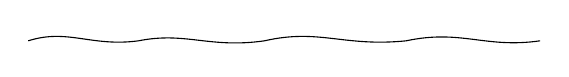
\begin{tikzpicture}\draw (0,0) .. controls (.5,.16) and (.8,-.08) .. (1.4,0) .. controls (2,.12) and (2.3,-.1) .. (3,0) .. controls (3.7,.16) and (4,-.08) .. (4.8,0) .. controls (5.5,.15) and (5.8,-.1) .. (6.5,0);\end{tikzpicture}}

Ça a l'air \unsure{fichtrement} compliqué comme présentation. Ne vaut il pas mieux dire ceci. Se donner une préfigure $\Phi$, c'est se donner

1°) $\Delta=\delta\Phi\in\mathrm{Drap}^{*}(\unsure{\mathcal{L}|L})$

2°) Une partie $\Phi_1\subset(\Phi_{\Delta})_1={}$ ens. des intervalles interstitiels de $\Delta$

3°) Une partie $\Phi_0\subset(\Phi_{\Delta})_0=\Delta$
\scanpage{127}
\mspage{118}
% archive sheet number: 127

\unsure{(}\uline{NB} Pour de telles données, la réunion $\Phi_0\cup\Phi_1$ est bien une figure, mais $\delta(\Phi_0\cup\Phi_1)\subset\Delta$ et l'inclusion peut être stricte, exemple : $\Phi_0=\Phi_1=\varnothing$ !\unsure{)} et il faut \unsure{lui|donc}, de plus poser une condition qui implique que $\delta(\Phi_0\cup\Phi_1)=\Delta$\unsure{\}}, \unsure{donc} avec la condition
\[
\unsure{\mathrm{Purfig}|\mathrm{Purifig}}_{\Delta}:\quad\forall s\in\Delta\setminus\deleted{\unsure{s}}\Phi_0,\quad\exists X\in\Phi_1\quad\text{t.q. }s\lhd X,
\]
en d'autres termes
\[
\deleted{\unsure{\Delta}}=\Phi_0\cup\bigcup_{X\in\Phi_1}\partial X\,.
\]
% slanted
\margin{\figure{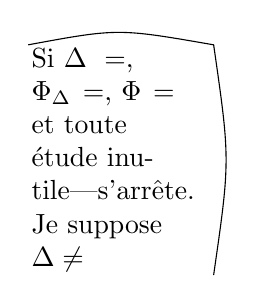
\begin{tikzpicture}
\node[inner sep=1pt,text width=2.2cm] (note) {Si $\Delta=\varnothing$, $\Phi_{\Delta}=\varnothing$, $\Phi=\varnothing$ et \unsure{toute} \unsure{étude} \unsure{inutile|s'arrête}. Je suppose $\Delta\ne\varnothing$};
\draw[thin] (note.north west) .. controls ([yshift=6pt]note.north) .. ([xshift=2pt]note.north east) .. controls ([xshift=8pt]note.east) .. ([xshift=2pt]note.south east);
\end{tikzpicture}}}

Considérons alors
\[
\begin{aligned}
\unsure{\Phi^{\prime *}|\Phi^{!*}}_0&=\deleted{\unsure{\Delta\setminus\Phi}}(\Phi_{\Delta})_0\setminus\Phi_0=\Delta\setminus\Phi_0\\
\Phi^{\prime *}_1&=(\Phi_{\Delta})_1\setminus\Phi_1
\end{aligned}
\]

Soit de plus, \deleted{si $\Delta\ne\varnothing$ (i.e. $\Phi\ne\varnothing$)}
\[
a=\mathrm{or}(\Delta),\quad b=\mathrm{ex}(\Delta)
\]
et soit
\[
\begin{aligned}
\unsure{\mathcal{M}|M}_{<a}&=\{X\in M\mid X<a\}\\
\mathcal{M}_{>b}&=\{X\in M\mid X>b\}
\end{aligned}
\]
Par Hyp., $\mathcal{M}_{<a}$ est $\varnothing$ sss $a$ est un plus petit élément de $\unsure{L|\mathcal{L}}$, et $\mathcal{M}_{>b}$ est vide \unsure{ssi|sss} $b$ est un plus grand élément de $L$. Ceci dit, on trouve \unsure{aussitôt}
\[
\mathrm{Cosupp}^{\circ}(\Phi)=\mathrm{Omb}^{\circ}(\Phi^{\prime *}_{\deleted{\unsure{1}}})\cup\mathcal{M}_{<a}\cup\mathcal{M}_{>b}
\]
(réunions disjointes), tandis que
\[
\mathrm{Omb}^{\circ}(\Phi^{\prime *})\overset{\mathrm{def}}{=}\bigcup_{X\in\Phi^{\prime *}}\mathrm{Omb}^{\circ}(X)
\]
\margin{\uline{réunion}\newline\uline{disjointe}}
